\documentclass[aspectratio=169,12pt]{beamer}
\usepackage[utf8]{inputenc}
\usepackage[english]{babel}
\usepackage{wrapfig}
%\usepackage{siunitx}

\usepackage{multicol}
\usepackage{mathtools}

\usepackage[normalem]{ulem}

\pagestyle{empty}

\usepackage{pgf,tikz}
\usepackage{pgfplots}
\usetikzlibrary{matrix}
\usetikzlibrary{arrows}

%\usepackage{wrapfig}
\mode<presentation>
\usefonttheme{professionalfonts}
\usetheme{Darmstadt}
\usecolortheme{orchid}
\useoutertheme{default}
\setbeamertemplate{headline}{}

\renewcommand{\baselinestretch}{1.1}

%gets rid of bottom navigation bars
\setbeamertemplate{footline}[page number]

%gets rid of navigation symbols
\setbeamertemplate{navigation symbols}{}

%\frameframe{none} % No default frame

%\setlength{\framewidth}{8.7in} \setlength{\frameheight}{7.2in}

\parindent 0pt
\setlength{\parskip} {1ex plus 0.5ex minus 0.2ex}


%\usepackage[bbgreekl]{mathbbol}
\usepackage{amsfonts}

%\DeclareSymbolFontAlphabet{\mathbb}{AMSb}
%\DeclareSymbolFontAlphabet{\mathbbl}{bbold}

\newcommand{\Sym}{{\mathcal S}}
\DeclareMathOperator{\Aut}{Aut}
\DeclareMathOperator{\Tr}{Tr}
\DeclareMathOperator{\trace}{Trace}
\DeclareMathOperator{\range}{range}
\DeclareMathOperator{\rank}{rank}

\usepackage{breqn}
\usepackage{multicol}
\usepackage{colortbl}
\usepackage{lmodern}
\usepackage{tabularx}
\usepackage{multirow}
\usepackage{amssymb}
\usepackage{amsmath}
\usepackage{stmaryrd}
\usepackage{color}
\usepackage{graphicx}
\graphicspath{ {img/} }
\usepackage{hyperref}

\input{epsf}
\title{Introducción}
\author{}

\DeclareMathOperator{\Hom}{Hom}
\DeclareMathOperator{\sing}{sing}

\DeclareMathOperator{\chara}{char}
\DeclareMathOperator{\Jacob}{Jacob}
\DeclareMathOperator{\Sing}{Sing}
\newcommand{\fracNoLine}[2]{\genfrac{}{}{}{0pt}{#1}{#2}}

%\beamerdefaultoverlayspecification{<+->}

\begin{document}

\newtheorem{prop}{Proposici\'on}
\newtheorem{algo}[prop]{Algorithm}
\newtheorem{teor}[prop]{Theorem}
\newtheorem{lema}[prop]{Lemma}
\newtheorem{coro}[prop]{Corollary}
\newtheorem{defi}[prop]{Definition}

\newcommand{\ideal}[1]{{\left\langle{#1}\right\rangle}}
\newcommand{\demo}{\textbf {Demostraci\'on. }}
\newcommand{\obse}{\textbf {Observaci\'on. }}
\newcommand{\Input}{\textbf {Input: }}
\newcommand{\Output}{\textbf {Output: }}
\newcommand{\Examp}{\textbf {Ejemplo }}
\newcommand{\Examps}{\textbf {Ejemplos }}

\newcommand{\kk}{{\mathbbl k}}
\newcommand{\V}{{\mathbf V}}
\newcommand{\I}{{\mathbf I}}
\newcommand{\PP}{{\tilde P}}
\newcommand{\QQ}{{\tilde Q}}

\newcommand{\F}{{\mathbb F}}
\newcommand{\Q}{{\mathbb Q}}
\newcommand{\N}{{\mathbb N}}
\newcommand{\R}{{\mathbb R}}
\newcommand{\Z}{{\mathbb Z}}
\newcommand{\CC}{{\mathbb C}}
\newcommand{\eLL}{{\mathcal L}}



\newcommand{\MinAss}{\textrm {MinAss}}
\newcommand{\Ass}{\textrm {Ass}}
\newcommand{\mcm}{\textrm {mcm}}
\newcommand{\mcd}{\textrm {mcd}}
%\newcommand{\mod}{\textrm { mod }}
\newcommand{\lt}{\textrm {lt}}
\newcommand{\Lt}{\textrm {Lt}}
\newcommand{\lp}{\textrm {lp}}
\newcommand{\lc}{\textrm {lc}}
\newcommand{\lm}{\textrm {lm}}
\newcommand{\barra}{\ /\ }
\newcommand{\multideg}{\textrm {multideg}}

\newcommand{\sep}{\textrm {sep}}
\newcommand{\Syz}{\textrm {Syz}}
\newcommand{\n}{\~n}
\newcommand{\cG}{\textrm {cG}}
\newcommand{\dG}{\textrm {dG}}
\newcommand{\nG}{\textrm {nG}}
\newcommand{\CE}{\textrm {CE}}
\newcommand{\CG}{\textrm {CG}}
\newcommand{\CF}{\textrm {CF}}
\newcommand{\DG}{\textrm {DG}}
\renewcommand{\NG}{\textrm {NG}}

\newcommand{\p}{{\boldsymbol{p}}}
\newcommand{\q}{{\boldsymbol{q}}}

\newcommand{\X}{{\boldsymbol{X}}}
\newcommand{\x}{{\boldsymbol{x}}}
\renewcommand{\u}{{\boldsymbol{u}}}
\renewcommand{\t}{{\boldsymbol{t}}}
\renewcommand{\a}{{\boldsymbol{a}}}
\renewcommand{\b}{{\boldsymbol{b}}}
\renewcommand{\c}{{\boldsymbol{c}}}

%Titulos en espa�ol
%\renewcommand{\chaptername}{Cap\'{\i}tulo}
%\renewcommand{\bibname}{Bibliograf\'{\i}a}

\newcommand{\kring}{\kk[\x]}
\newcommand{\kRing}{\kk[X]}
\newcommand{\qring}{\Q[\x]}

%\renewcommand\itemindent{-10pt}
%\renewcommand{\theenumi}{\arabic{enumi}}
%\renewcommand{\labelenumi}{\Alph{enumi}}

\definecolor{issac}{rgb}{1.00,0.00,0.00}
%------------------------------------------------------------------

\begin{frame}

 \begin{center}

\Large\textbf{Laboratorio de Datos} \\
\large\textbf{Estadística descriptiva}
%\vspace{0.5cm}

% \textit{Santiago Laplagne} \\
%slaplagn@dm.uba.ar \\


%\vspace{0.5cm}
%{\small Trabajo en progreso en conjunto con \emph{Jose Capco} (Universit\"at Innsbruck) y \emph{Claus Scheiderer} %(Universit\"at Konstanz).} \\

\vspace{1cm}
Primer Cuatrimestre 2024 \\ Turnos tarde y noche

\vspace{1cm}


 {\small Facultad de Ciencias Exactas y Naturales, UBA}
 \end{center}


\end{frame}

%------------------------------------------------------------------

\begin{frame}
\frametitle{Variables Categóricas vs Numéricas}
\begin{block}{Variables Categóricas}
Son variables que representan diferentes categorías o grupos. 
Las variables categóricas se pueden dividir en dos tipos: nominal y ordinal.
\begin{itemize}
    \item \textbf{Nominal:} No tienen un orden intrínseco.
    \item \textbf{Ordinal:} Tienen un orden intrínseco.
\end{itemize}
\end{block}
\end{frame}

%------------------------------------------------------------------

\begin{frame}
\frametitle{Ejemplos}
\begin{itemize}
    \item \textbf{Variable Categórica:}
    \begin{itemize}
        \item Nominal: Color de los ojos
        \begin{itemize}
            \item Azul
            \item Marrón
            \item Verde
            \item Gris
        \end{itemize}
        \item Ordinal: Nivel de educación
        \begin{itemize}
            \item Primaria
            \item Secundaria
            \item Universitaria
            \item Posgrado
        \end{itemize}
    \end{itemize}
\end{itemize}

\end{frame}

%------------------------------------------------------------------

\begin{frame}
\frametitle{Variables Categóricas vs Numéricas}
\begin{block}{Variables Numéricas}
Son variables que representan cantidades numéricas.
Las variables numéricas se pueden dividir en dos tipos: discreta y continua.
\begin{itemize}
    \item \textbf{Discreta:} Representa valores contables y no puede tomar valores intermedios.
    \item \textbf{Continua:} Representa medidas y puede tomar cualquier valor dentro de un rango.
\end{itemize}
\end{block}

\end{frame}

%------------------------------------------------------------------
%
%\begin{frame}
%\frametitle{Modelos lineales}
%
%
%\end{frame}
%
%------------------------------------------------------------------

\begin{frame}
\frametitle{Ejemplos}
\begin{itemize}
    \item \textbf{Variable Numérica:}
    \begin{itemize}
        \item Discreta: Número de hijos
        \begin{itemize}
            \item 0
            \item 1
            \item 2
            \item 3
        \end{itemize}
        \item Continua: Altura (en metros)
        \begin{itemize}
            \item 1.60
            \item 1.75
            \item 1.82
            \item 1.68
        \end{itemize}
    \end{itemize}
\end{itemize}

\end{frame}


%------------------------------------------------------------------

\begin{frame}
\frametitle{Medidas de tendencia central: media y mediana}
\begin{block}{Media}
La media es el promedio de un conjunto de datos y se calcula sumando todos los valores y dividiéndolos por el número total de valores.
\[ \text{Media} = \frac{x_1 + x_2 + \dots + x_n}{n} = \frac{\sum_{i=1}^{n} x_i}{n} \]
\end{block}

\begin{block}{Mediana}
La mediana es el valor del medio cuando un conjunto de datos se ordena de menor a mayor. Si hay una cantidad par de datos, se toma el promedio entre los dos valores del medio.
\end{block}
\end{frame}

%------------------------------------------------------------------

\begin{frame}
\frametitle{Ejemplos Numéricos}
\begin{block}{Conjunto de datos 1: $2, 6, 8, 10, 9$}
\begin{itemize}
    \item Media:
    \[ \frac{2+6+8+10+9}{5} = \frac{35}{5} = 7 \]
    \item Mediana: ordenamos de menor a mayor $2, 6, 8, 9, 10$
    
    La mediana es 8.
\end{itemize}
\end{block}

\begin{block}{Conjunto de datos 2: $2, 6, 8, 50, 9$}
\begin{itemize}
    \item Media:
    \[ \frac{2+6+8+50+9}{5} = \frac{75}{5} = 15 \]
    \item Mediana: ordenamos de menor a mayor $2, 6, 8, 9, 50$
    
    La mediana es 8.
\end{itemize}
\end{block}
\end{frame}

\begin{frame}
\frametitle{Diferencia entre Media y Mediana: Outliers}

Un outlier o valor atípico es una observación dentro de una muestra que no es consistente con el resto.

\begin{block}{Media}
La media es sensible a los valores atípicos (outliers), ya que se calcula sumando todos los valores y dividiéndolos por el número total de valores.
\begin{itemize}
    \item Si hay outliers, la media puede sesgarse significativamente hacia los valores extremos.
\end{itemize}
\end{block}

\begin{block}{Mediana}
La mediana no se ve afectada por los valores atípicos, ya que es el valor central de un conjunto de datos ordenados.
\begin{itemize}
    \item Es más robusta frente a valores extremos que la media.
\end{itemize}
\end{block}
\end{frame}

%------------------------------------------------------------------

\begin{frame}
\frametitle{Media y mediana}

\begin{center}
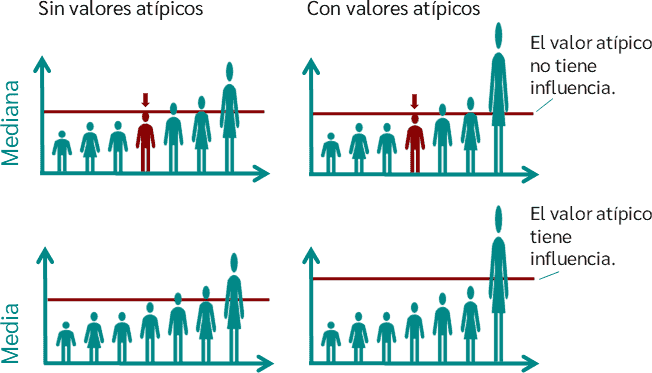
\includegraphics[scale=0.6]{clase2-img-alturas.png}
\end{center}
\end{frame}

%------------------------------------------------------------------

\begin{frame}
\frametitle{Varianza y desvío Estándar}
\begin{block}{Definición}
La varianza y el desvío estándar son \emph{medidas de dispersión} que indican cuánto varían los valores de un conjunto de datos respecto a la media.
\end{block}

\begin{block}{Fórmula}
La varianza se calcula mediante la fórmula:
\[ \text{varianza} = \frac{\sum_{i=1}^{n}(x_i - \mu)^2}{n}, \]
donde $\mu$ es la media de los datos.

El desvío se calcula como la raíz cuadrada de la varianza:
\[ \sigma = \sqrt{\frac{\sum_{i=1}^{n}(x_i - \mu)^2}{n}}. \]
\end{block}
\end{frame}

\begin{frame}
\frametitle{Interpretación}
\begin{itemize}
    \item Un desvío estándar pequeño indica que los datos están cercanos a la media.
    \item Un desvío estándar grande indica que los datos están dispersos y alejados de la media.
\end{itemize}

\begin{block}{Ejemplo}
Consideramos el siguiente conjunto de datos: $1, 2, 3, 4, 5$
\begin{itemize}
    \item Media ($\mu$): 3
    \item Varianza: $\frac{2^2 + 1^2 + 0 + 1^2 + 2^2}{5} = 2$
    \item Desvío Estándar ($\sigma$): $\sqrt{2} = 1.41$
\end{itemize}
\end{block}
\end{frame}

%------------------------------------------------------------------

\end{document}

